% Created by tikzDevice version 0.6.2-92-0ad2792 on 2013-03-04 10:17:45
% !TEX encoding = UTF-8 Unicode
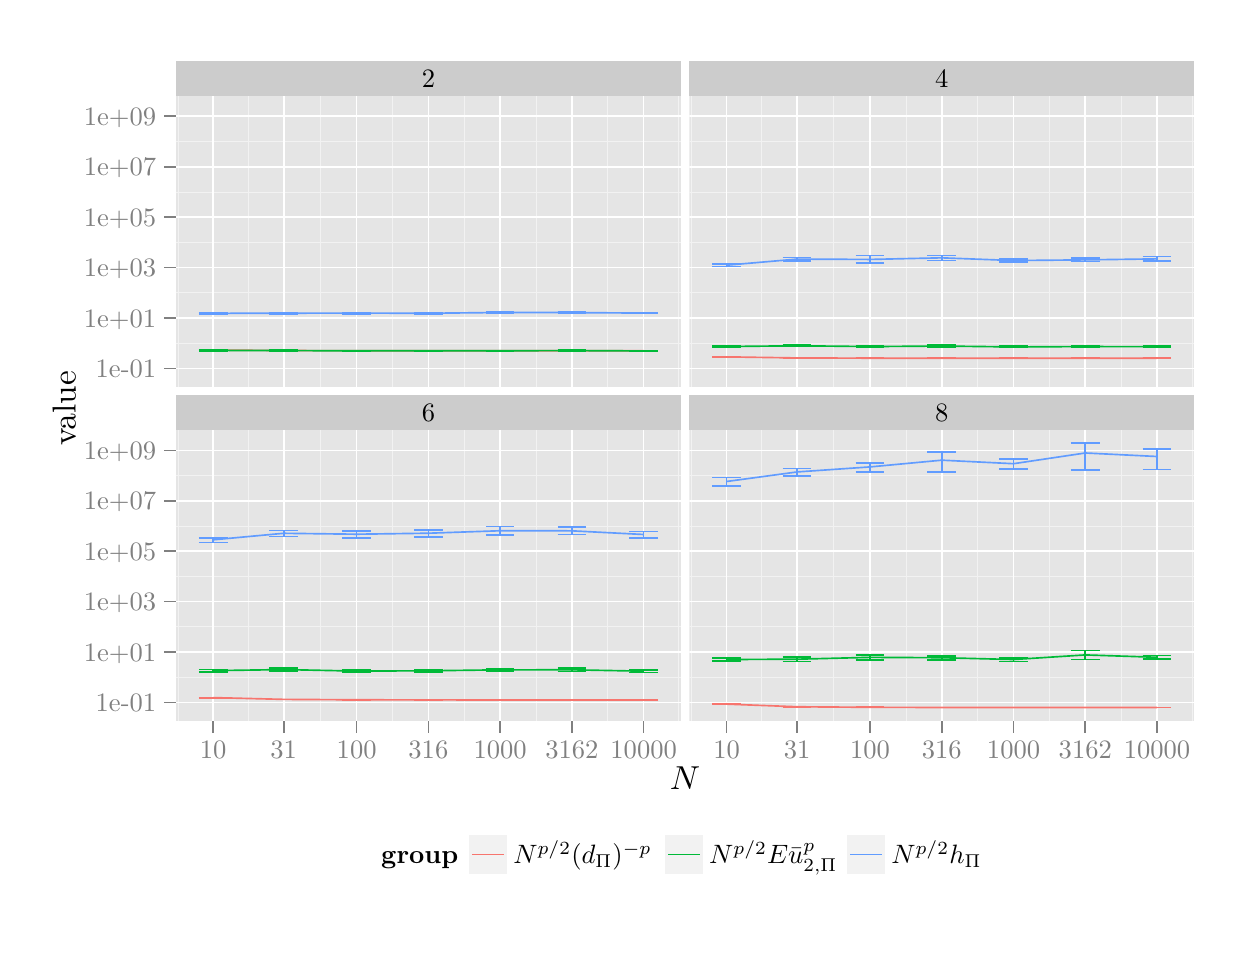
\begin{tikzpicture}[x=1pt,y=1pt]
\definecolor[named]{fillColor}{rgb}{1.00,1.00,1.00}
\path[use as bounding box,fill=fillColor,fill opacity=0.00] (0,0) rectangle (433.62,325.21);
\begin{scope}
\path[clip] (  0.00,  0.00) rectangle (433.62,325.21);
\definecolor[named]{drawColor}{rgb}{1.00,1.00,1.00}
\definecolor[named]{fillColor}{rgb}{1.00,1.00,1.00}

\path[draw=drawColor,line width= 0.6pt,line join=round,line cap=round,fill=fillColor] (  0.00,  0.00) rectangle (433.62,325.21);
\end{scope}
\begin{scope}
\path[clip] ( 53.55,195.47) rectangle (236.06,300.54);
\definecolor[named]{fillColor}{rgb}{0.90,0.90,0.90}

\path[fill=fillColor] ( 53.55,195.47) rectangle (236.06,300.54);
\definecolor[named]{drawColor}{rgb}{0.95,0.95,0.95}

\path[draw=drawColor,line width= 0.3pt,line join=round] ( 53.55,211.21) --
	(236.06,211.21);

\path[draw=drawColor,line width= 0.3pt,line join=round] ( 53.55,229.42) --
	(236.06,229.42);

\path[draw=drawColor,line width= 0.3pt,line join=round] ( 53.55,247.64) --
	(236.06,247.64);

\path[draw=drawColor,line width= 0.3pt,line join=round] ( 53.55,265.85) --
	(236.06,265.85);

\path[draw=drawColor,line width= 0.3pt,line join=round] ( 53.55,284.06) --
	(236.06,284.06);

\path[draw=drawColor,line width= 0.3pt,line join=round] ( 54.29,195.47) --
	( 54.29,300.54);

\path[draw=drawColor,line width= 0.3pt,line join=round] ( 79.77,195.47) --
	( 79.77,300.54);

\path[draw=drawColor,line width= 0.3pt,line join=round] (105.69,195.47) --
	(105.69,300.54);

\path[draw=drawColor,line width= 0.3pt,line join=round] (131.83,195.47) --
	(131.83,300.54);

\path[draw=drawColor,line width= 0.3pt,line join=round] (157.76,195.47) --
	(157.76,300.54);

\path[draw=drawColor,line width= 0.3pt,line join=round] (183.69,195.47) --
	(183.69,300.54);

\path[draw=drawColor,line width= 0.3pt,line join=round] (209.61,195.47) --
	(209.61,300.54);

\path[draw=drawColor,line width= 0.3pt,line join=round] (235.31,195.47) --
	(235.31,300.54);
\definecolor[named]{drawColor}{rgb}{1.00,1.00,1.00}

\path[draw=drawColor,line width= 0.6pt,line join=round] ( 53.55,202.10) --
	(236.06,202.10);

\path[draw=drawColor,line width= 0.6pt,line join=round] ( 53.55,220.32) --
	(236.06,220.32);

\path[draw=drawColor,line width= 0.6pt,line join=round] ( 53.55,238.53) --
	(236.06,238.53);

\path[draw=drawColor,line width= 0.6pt,line join=round] ( 53.55,256.74) --
	(236.06,256.74);

\path[draw=drawColor,line width= 0.6pt,line join=round] ( 53.55,274.95) --
	(236.06,274.95);

\path[draw=drawColor,line width= 0.6pt,line join=round] ( 53.55,293.17) --
	(236.06,293.17);

\path[draw=drawColor,line width= 0.6pt,line join=round] ( 67.03,195.47) --
	( 67.03,300.54);

\path[draw=drawColor,line width= 0.6pt,line join=round] ( 92.51,195.47) --
	( 92.51,300.54);

\path[draw=drawColor,line width= 0.6pt,line join=round] (118.88,195.47) --
	(118.88,300.54);

\path[draw=drawColor,line width= 0.6pt,line join=round] (144.79,195.47) --
	(144.79,300.54);

\path[draw=drawColor,line width= 0.6pt,line join=round] (170.73,195.47) --
	(170.73,300.54);

\path[draw=drawColor,line width= 0.6pt,line join=round] (196.65,195.47) --
	(196.65,300.54);

\path[draw=drawColor,line width= 0.6pt,line join=round] (222.58,195.47) --
	(222.58,300.54);
\definecolor[named]{drawColor}{rgb}{0.97,0.46,0.43}

\path[draw=drawColor,line width= 0.6pt,line join=round] ( 67.03,208.71) --
	( 92.51,208.54) --
	(118.88,208.49) --
	(144.79,208.48) --
	(170.73,208.47) --
	(196.65,208.47) --
	(222.58,208.47);
\definecolor[named]{drawColor}{rgb}{0.00,0.73,0.22}

\path[draw=drawColor,line width= 0.6pt,line join=round] ( 67.03,208.60) --
	( 92.51,208.52) --
	(118.88,208.45) --
	(144.79,208.49) --
	(170.73,208.46) --
	(196.65,208.52) --
	(222.58,208.40);
\definecolor[named]{drawColor}{rgb}{0.38,0.61,1.00}

\path[draw=drawColor,line width= 0.6pt,line join=round] ( 67.03,221.97) --
	( 92.51,222.03) --
	(118.88,222.07) --
	(144.79,222.01) --
	(170.73,222.29) --
	(196.65,222.25) --
	(222.58,222.08);
\definecolor[named]{drawColor}{rgb}{0.97,0.46,0.43}

\path[draw=drawColor,line width= 0.6pt,line join=round] ( 61.85,208.72) --
	( 72.22,208.72);

\path[draw=drawColor,line width= 0.6pt,line join=round] ( 67.03,208.72) --
	( 67.03,208.70);

\path[draw=drawColor,line width= 0.6pt,line join=round] ( 61.85,208.70) --
	( 72.22,208.70);

\path[draw=drawColor,line width= 0.6pt,line join=round] ( 87.32,208.54) --
	( 97.69,208.54);

\path[draw=drawColor,line width= 0.6pt,line join=round] ( 92.51,208.54) --
	( 92.51,208.53);

\path[draw=drawColor,line width= 0.6pt,line join=round] ( 87.32,208.53) --
	( 97.69,208.53);

\path[draw=drawColor,line width= 0.6pt,line join=round] (113.69,208.49) --
	(124.06,208.49);

\path[draw=drawColor,line width= 0.6pt,line join=round] (118.88,208.49) --
	(118.88,208.49);

\path[draw=drawColor,line width= 0.6pt,line join=round] (113.69,208.49) --
	(124.06,208.49);

\path[draw=drawColor,line width= 0.6pt,line join=round] (139.60,208.48) --
	(149.97,208.48);

\path[draw=drawColor,line width= 0.6pt,line join=round] (144.79,208.48) --
	(144.79,208.48);

\path[draw=drawColor,line width= 0.6pt,line join=round] (139.60,208.48) --
	(149.97,208.48);

\path[draw=drawColor,line width= 0.6pt,line join=round] (165.54,208.47) --
	(175.91,208.47);

\path[draw=drawColor,line width= 0.6pt,line join=round] (170.73,208.47) --
	(170.73,208.47);

\path[draw=drawColor,line width= 0.6pt,line join=round] (165.54,208.47) --
	(175.91,208.47);

\path[draw=drawColor,line width= 0.6pt,line join=round] (191.47,208.47) --
	(201.83,208.47);

\path[draw=drawColor,line width= 0.6pt,line join=round] (196.65,208.47) --
	(196.65,208.47);

\path[draw=drawColor,line width= 0.6pt,line join=round] (191.47,208.47) --
	(201.83,208.47);

\path[draw=drawColor,line width= 0.6pt,line join=round] (217.39,208.47) --
	(227.76,208.47);

\path[draw=drawColor,line width= 0.6pt,line join=round] (222.58,208.47) --
	(222.58,208.47);

\path[draw=drawColor,line width= 0.6pt,line join=round] (217.39,208.47) --
	(227.76,208.47);
\definecolor[named]{drawColor}{rgb}{0.00,0.73,0.22}

\path[draw=drawColor,line width= 0.6pt,line join=round] ( 61.85,208.71) --
	( 72.22,208.71);

\path[draw=drawColor,line width= 0.6pt,line join=round] ( 67.03,208.71) --
	( 67.03,208.49);

\path[draw=drawColor,line width= 0.6pt,line join=round] ( 61.85,208.49) --
	( 72.22,208.49);

\path[draw=drawColor,line width= 0.6pt,line join=round] ( 87.32,208.63) --
	( 97.69,208.63);

\path[draw=drawColor,line width= 0.6pt,line join=round] ( 92.51,208.63) --
	( 92.51,208.42);

\path[draw=drawColor,line width= 0.6pt,line join=round] ( 87.32,208.42) --
	( 97.69,208.42);

\path[draw=drawColor,line width= 0.6pt,line join=round] (113.69,208.56) --
	(124.06,208.56);

\path[draw=drawColor,line width= 0.6pt,line join=round] (118.88,208.56) --
	(118.88,208.34);

\path[draw=drawColor,line width= 0.6pt,line join=round] (113.69,208.34) --
	(124.06,208.34);

\path[draw=drawColor,line width= 0.6pt,line join=round] (139.60,208.59) --
	(149.97,208.59);

\path[draw=drawColor,line width= 0.6pt,line join=round] (144.79,208.59) --
	(144.79,208.38);

\path[draw=drawColor,line width= 0.6pt,line join=round] (139.60,208.38) --
	(149.97,208.38);

\path[draw=drawColor,line width= 0.6pt,line join=round] (165.54,208.56) --
	(175.91,208.56);

\path[draw=drawColor,line width= 0.6pt,line join=round] (170.73,208.56) --
	(170.73,208.35);

\path[draw=drawColor,line width= 0.6pt,line join=round] (165.54,208.35) --
	(175.91,208.35);

\path[draw=drawColor,line width= 0.6pt,line join=round] (191.47,208.63) --
	(201.83,208.63);

\path[draw=drawColor,line width= 0.6pt,line join=round] (196.65,208.63) --
	(196.65,208.41);

\path[draw=drawColor,line width= 0.6pt,line join=round] (191.47,208.41) --
	(201.83,208.41);

\path[draw=drawColor,line width= 0.6pt,line join=round] (217.39,208.50) --
	(227.76,208.50);

\path[draw=drawColor,line width= 0.6pt,line join=round] (222.58,208.50) --
	(222.58,208.28);

\path[draw=drawColor,line width= 0.6pt,line join=round] (217.39,208.28) --
	(227.76,208.28);
\definecolor[named]{drawColor}{rgb}{0.38,0.61,1.00}

\path[draw=drawColor,line width= 0.6pt,line join=round] ( 61.85,222.13) --
	( 72.22,222.13);

\path[draw=drawColor,line width= 0.6pt,line join=round] ( 67.03,222.13) --
	( 67.03,221.81);

\path[draw=drawColor,line width= 0.6pt,line join=round] ( 61.85,221.81) --
	( 72.22,221.81);

\path[draw=drawColor,line width= 0.6pt,line join=round] ( 87.32,222.22) --
	( 97.69,222.22);

\path[draw=drawColor,line width= 0.6pt,line join=round] ( 92.51,222.22) --
	( 92.51,221.84);

\path[draw=drawColor,line width= 0.6pt,line join=round] ( 87.32,221.84) --
	( 97.69,221.84);

\path[draw=drawColor,line width= 0.6pt,line join=round] (113.69,222.26) --
	(124.06,222.26);

\path[draw=drawColor,line width= 0.6pt,line join=round] (118.88,222.26) --
	(118.88,221.86);

\path[draw=drawColor,line width= 0.6pt,line join=round] (113.69,221.86) --
	(124.06,221.86);

\path[draw=drawColor,line width= 0.6pt,line join=round] (139.60,222.21) --
	(149.97,222.21);

\path[draw=drawColor,line width= 0.6pt,line join=round] (144.79,222.21) --
	(144.79,221.80);

\path[draw=drawColor,line width= 0.6pt,line join=round] (139.60,221.80) --
	(149.97,221.80);

\path[draw=drawColor,line width= 0.6pt,line join=round] (165.54,222.49) --
	(175.91,222.49);

\path[draw=drawColor,line width= 0.6pt,line join=round] (170.73,222.49) --
	(170.73,222.07);

\path[draw=drawColor,line width= 0.6pt,line join=round] (165.54,222.07) --
	(175.91,222.07);

\path[draw=drawColor,line width= 0.6pt,line join=round] (191.47,222.46) --
	(201.83,222.46);

\path[draw=drawColor,line width= 0.6pt,line join=round] (196.65,222.46) --
	(196.65,222.03);

\path[draw=drawColor,line width= 0.6pt,line join=round] (191.47,222.03) --
	(201.83,222.03);

\path[draw=drawColor,line width= 0.6pt,line join=round] (217.39,222.28) --
	(227.76,222.28);

\path[draw=drawColor,line width= 0.6pt,line join=round] (222.58,222.28) --
	(222.58,221.88);

\path[draw=drawColor,line width= 0.6pt,line join=round] (217.39,221.88) --
	(227.76,221.88);
\end{scope}
\begin{scope}
\path[clip] (239.07,195.47) rectangle (421.58,300.54);
\definecolor[named]{fillColor}{rgb}{0.90,0.90,0.90}

\path[fill=fillColor] (239.07,195.47) rectangle (421.57,300.54);
\definecolor[named]{drawColor}{rgb}{0.95,0.95,0.95}

\path[draw=drawColor,line width= 0.3pt,line join=round] (239.07,211.21) --
	(421.58,211.21);

\path[draw=drawColor,line width= 0.3pt,line join=round] (239.07,229.42) --
	(421.58,229.42);

\path[draw=drawColor,line width= 0.3pt,line join=round] (239.07,247.64) --
	(421.58,247.64);

\path[draw=drawColor,line width= 0.3pt,line join=round] (239.07,265.85) --
	(421.58,265.85);

\path[draw=drawColor,line width= 0.3pt,line join=round] (239.07,284.06) --
	(421.58,284.06);

\path[draw=drawColor,line width= 0.3pt,line join=round] (239.81,195.47) --
	(239.81,300.54);

\path[draw=drawColor,line width= 0.3pt,line join=round] (265.29,195.47) --
	(265.29,300.54);

\path[draw=drawColor,line width= 0.3pt,line join=round] (291.21,195.47) --
	(291.21,300.54);

\path[draw=drawColor,line width= 0.3pt,line join=round] (317.35,195.47) --
	(317.35,300.54);

\path[draw=drawColor,line width= 0.3pt,line join=round] (343.28,195.47) --
	(343.28,300.54);

\path[draw=drawColor,line width= 0.3pt,line join=round] (369.21,195.47) --
	(369.21,300.54);

\path[draw=drawColor,line width= 0.3pt,line join=round] (395.13,195.47) --
	(395.13,300.54);

\path[draw=drawColor,line width= 0.3pt,line join=round] (420.83,195.47) --
	(420.83,300.54);
\definecolor[named]{drawColor}{rgb}{1.00,1.00,1.00}

\path[draw=drawColor,line width= 0.6pt,line join=round] (239.07,202.10) --
	(421.58,202.10);

\path[draw=drawColor,line width= 0.6pt,line join=round] (239.07,220.32) --
	(421.58,220.32);

\path[draw=drawColor,line width= 0.6pt,line join=round] (239.07,238.53) --
	(421.58,238.53);

\path[draw=drawColor,line width= 0.6pt,line join=round] (239.07,256.74) --
	(421.58,256.74);

\path[draw=drawColor,line width= 0.6pt,line join=round] (239.07,274.95) --
	(421.58,274.95);

\path[draw=drawColor,line width= 0.6pt,line join=round] (239.07,293.17) --
	(421.58,293.17);

\path[draw=drawColor,line width= 0.6pt,line join=round] (252.55,195.47) --
	(252.55,300.54);

\path[draw=drawColor,line width= 0.6pt,line join=round] (278.03,195.47) --
	(278.03,300.54);

\path[draw=drawColor,line width= 0.6pt,line join=round] (304.40,195.47) --
	(304.40,300.54);

\path[draw=drawColor,line width= 0.6pt,line join=round] (330.31,195.47) --
	(330.31,300.54);

\path[draw=drawColor,line width= 0.6pt,line join=round] (356.25,195.47) --
	(356.25,300.54);

\path[draw=drawColor,line width= 0.6pt,line join=round] (382.17,195.47) --
	(382.17,300.54);

\path[draw=drawColor,line width= 0.6pt,line join=round] (408.09,195.47) --
	(408.09,300.54);
\definecolor[named]{drawColor}{rgb}{0.97,0.46,0.43}

\path[draw=drawColor,line width= 0.6pt,line join=round] (252.55,206.24) --
	(278.03,205.87) --
	(304.40,205.77) --
	(330.31,205.74) --
	(356.25,205.73) --
	(382.17,205.73) --
	(408.09,205.73);
\definecolor[named]{drawColor}{rgb}{0.00,0.73,0.22}

\path[draw=drawColor,line width= 0.6pt,line join=round] (252.55,209.99) --
	(278.03,210.26) --
	(304.40,209.98) --
	(330.31,210.16) --
	(356.25,209.85) --
	(382.17,209.98) --
	(408.09,209.94);
\definecolor[named]{drawColor}{rgb}{0.38,0.61,1.00}

\path[draw=drawColor,line width= 0.6pt,line join=round] (252.55,239.38) --
	(278.03,241.58) --
	(304.40,241.46) --
	(330.31,242.04) --
	(356.25,241.06) --
	(382.17,241.30) --
	(408.09,241.66);
\definecolor[named]{drawColor}{rgb}{0.97,0.46,0.43}

\path[draw=drawColor,line width= 0.6pt,line join=round] (247.36,206.25) --
	(257.73,206.25);

\path[draw=drawColor,line width= 0.6pt,line join=round] (252.55,206.25) --
	(252.55,206.22);

\path[draw=drawColor,line width= 0.6pt,line join=round] (247.36,206.22) --
	(257.73,206.22);

\path[draw=drawColor,line width= 0.6pt,line join=round] (272.84,205.87) --
	(283.21,205.87);

\path[draw=drawColor,line width= 0.6pt,line join=round] (278.03,205.87) --
	(278.03,205.86);

\path[draw=drawColor,line width= 0.6pt,line join=round] (272.84,205.86) --
	(283.21,205.86);

\path[draw=drawColor,line width= 0.6pt,line join=round] (299.21,205.77) --
	(309.58,205.77);

\path[draw=drawColor,line width= 0.6pt,line join=round] (304.40,205.77) --
	(304.40,205.77);

\path[draw=drawColor,line width= 0.6pt,line join=round] (299.21,205.77) --
	(309.58,205.77);

\path[draw=drawColor,line width= 0.6pt,line join=round] (325.12,205.74) --
	(335.49,205.74);

\path[draw=drawColor,line width= 0.6pt,line join=round] (330.31,205.74) --
	(330.31,205.74);

\path[draw=drawColor,line width= 0.6pt,line join=round] (325.12,205.74) --
	(335.49,205.74);

\path[draw=drawColor,line width= 0.6pt,line join=round] (351.06,205.73) --
	(361.43,205.73);

\path[draw=drawColor,line width= 0.6pt,line join=round] (356.25,205.73) --
	(356.25,205.73);

\path[draw=drawColor,line width= 0.6pt,line join=round] (351.06,205.73) --
	(361.43,205.73);

\path[draw=drawColor,line width= 0.6pt,line join=round] (376.98,205.73) --
	(387.35,205.73);

\path[draw=drawColor,line width= 0.6pt,line join=round] (382.17,205.73) --
	(382.17,205.73);

\path[draw=drawColor,line width= 0.6pt,line join=round] (376.98,205.73) --
	(387.35,205.73);

\path[draw=drawColor,line width= 0.6pt,line join=round] (402.91,205.73) --
	(413.28,205.73);

\path[draw=drawColor,line width= 0.6pt,line join=round] (408.09,205.73) --
	(408.09,205.73);

\path[draw=drawColor,line width= 0.6pt,line join=round] (402.91,205.73) --
	(413.28,205.73);
\definecolor[named]{drawColor}{rgb}{0.00,0.73,0.22}

\path[draw=drawColor,line width= 0.6pt,line join=round] (247.36,210.20) --
	(257.73,210.20);

\path[draw=drawColor,line width= 0.6pt,line join=round] (252.55,210.20) --
	(252.55,209.79);

\path[draw=drawColor,line width= 0.6pt,line join=round] (247.36,209.79) --
	(257.73,209.79);

\path[draw=drawColor,line width= 0.6pt,line join=round] (272.84,210.50) --
	(283.21,210.50);

\path[draw=drawColor,line width= 0.6pt,line join=round] (278.03,210.50) --
	(278.03,210.00);

\path[draw=drawColor,line width= 0.6pt,line join=round] (272.84,210.00) --
	(283.21,210.00);

\path[draw=drawColor,line width= 0.6pt,line join=round] (299.21,210.22) --
	(309.58,210.22);

\path[draw=drawColor,line width= 0.6pt,line join=round] (304.40,210.22) --
	(304.40,209.73);

\path[draw=drawColor,line width= 0.6pt,line join=round] (299.21,209.73) --
	(309.58,209.73);

\path[draw=drawColor,line width= 0.6pt,line join=round] (325.12,210.43) --
	(335.49,210.43);

\path[draw=drawColor,line width= 0.6pt,line join=round] (330.31,210.43) --
	(330.31,209.91);

\path[draw=drawColor,line width= 0.6pt,line join=round] (325.12,209.91) --
	(335.49,209.91);

\path[draw=drawColor,line width= 0.6pt,line join=round] (351.06,210.07) --
	(361.43,210.07);

\path[draw=drawColor,line width= 0.6pt,line join=round] (356.25,210.07) --
	(356.25,209.60);

\path[draw=drawColor,line width= 0.6pt,line join=round] (351.06,209.60) --
	(361.43,209.60);

\path[draw=drawColor,line width= 0.6pt,line join=round] (376.98,210.25) --
	(387.35,210.25);

\path[draw=drawColor,line width= 0.6pt,line join=round] (382.17,210.25) --
	(382.17,209.72);

\path[draw=drawColor,line width= 0.6pt,line join=round] (376.98,209.72) --
	(387.35,209.72);

\path[draw=drawColor,line width= 0.6pt,line join=round] (402.91,210.18) --
	(413.28,210.18);

\path[draw=drawColor,line width= 0.6pt,line join=round] (408.09,210.18) --
	(408.09,209.67);

\path[draw=drawColor,line width= 0.6pt,line join=round] (402.91,209.67) --
	(413.28,209.67);
\definecolor[named]{drawColor}{rgb}{0.38,0.61,1.00}

\path[draw=drawColor,line width= 0.6pt,line join=round] (247.36,239.83) --
	(257.73,239.83);

\path[draw=drawColor,line width= 0.6pt,line join=round] (252.55,239.83) --
	(252.55,238.93);

\path[draw=drawColor,line width= 0.6pt,line join=round] (247.36,238.93) --
	(257.73,238.93);

\path[draw=drawColor,line width= 0.6pt,line join=round] (272.84,242.18) --
	(283.21,242.18);

\path[draw=drawColor,line width= 0.6pt,line join=round] (278.03,242.18) --
	(278.03,240.93);

\path[draw=drawColor,line width= 0.6pt,line join=round] (272.84,240.93) --
	(283.21,240.93);

\path[draw=drawColor,line width= 0.6pt,line join=round] (299.21,242.89) --
	(309.58,242.89);

\path[draw=drawColor,line width= 0.6pt,line join=round] (304.40,242.89) --
	(304.40,240.21);

\path[draw=drawColor,line width= 0.6pt,line join=round] (299.21,240.21) --
	(309.58,240.21);

\path[draw=drawColor,line width= 0.6pt,line join=round] (325.12,242.93) --
	(335.49,242.93);

\path[draw=drawColor,line width= 0.6pt,line join=round] (330.31,242.93) --
	(330.31,241.08);

\path[draw=drawColor,line width= 0.6pt,line join=round] (325.12,241.08) --
	(335.49,241.08);

\path[draw=drawColor,line width= 0.6pt,line join=round] (351.06,241.60) --
	(361.43,241.60);

\path[draw=drawColor,line width= 0.6pt,line join=round] (356.25,241.60) --
	(356.25,240.45);

\path[draw=drawColor,line width= 0.6pt,line join=round] (351.06,240.45) --
	(361.43,240.45);

\path[draw=drawColor,line width= 0.6pt,line join=round] (376.98,241.92) --
	(387.35,241.92);

\path[draw=drawColor,line width= 0.6pt,line join=round] (382.17,241.92) --
	(382.17,240.69);

\path[draw=drawColor,line width= 0.6pt,line join=round] (376.98,240.69) --
	(387.35,240.69);

\path[draw=drawColor,line width= 0.6pt,line join=round] (402.91,242.52) --
	(413.28,242.52);

\path[draw=drawColor,line width= 0.6pt,line join=round] (408.09,242.52) --
	(408.09,240.85);

\path[draw=drawColor,line width= 0.6pt,line join=round] (402.91,240.85) --
	(413.28,240.85);
\end{scope}
\begin{scope}
\path[clip] ( 53.55, 74.76) rectangle (236.06,179.83);
\definecolor[named]{fillColor}{rgb}{0.90,0.90,0.90}

\path[fill=fillColor] ( 53.55, 74.76) rectangle (236.06,179.83);
\definecolor[named]{drawColor}{rgb}{0.95,0.95,0.95}

\path[draw=drawColor,line width= 0.3pt,line join=round] ( 53.55, 90.50) --
	(236.06, 90.50);

\path[draw=drawColor,line width= 0.3pt,line join=round] ( 53.55,108.71) --
	(236.06,108.71);

\path[draw=drawColor,line width= 0.3pt,line join=round] ( 53.55,126.93) --
	(236.06,126.93);

\path[draw=drawColor,line width= 0.3pt,line join=round] ( 53.55,145.14) --
	(236.06,145.14);

\path[draw=drawColor,line width= 0.3pt,line join=round] ( 53.55,163.35) --
	(236.06,163.35);

\path[draw=drawColor,line width= 0.3pt,line join=round] ( 54.29, 74.76) --
	( 54.29,179.83);

\path[draw=drawColor,line width= 0.3pt,line join=round] ( 79.77, 74.76) --
	( 79.77,179.83);

\path[draw=drawColor,line width= 0.3pt,line join=round] (105.69, 74.76) --
	(105.69,179.83);

\path[draw=drawColor,line width= 0.3pt,line join=round] (131.83, 74.76) --
	(131.83,179.83);

\path[draw=drawColor,line width= 0.3pt,line join=round] (157.76, 74.76) --
	(157.76,179.83);

\path[draw=drawColor,line width= 0.3pt,line join=round] (183.69, 74.76) --
	(183.69,179.83);

\path[draw=drawColor,line width= 0.3pt,line join=round] (209.61, 74.76) --
	(209.61,179.83);

\path[draw=drawColor,line width= 0.3pt,line join=round] (235.31, 74.76) --
	(235.31,179.83);
\definecolor[named]{drawColor}{rgb}{1.00,1.00,1.00}

\path[draw=drawColor,line width= 0.6pt,line join=round] ( 53.55, 81.39) --
	(236.06, 81.39);

\path[draw=drawColor,line width= 0.6pt,line join=round] ( 53.55, 99.61) --
	(236.06, 99.61);

\path[draw=drawColor,line width= 0.6pt,line join=round] ( 53.55,117.82) --
	(236.06,117.82);

\path[draw=drawColor,line width= 0.6pt,line join=round] ( 53.55,136.03) --
	(236.06,136.03);

\path[draw=drawColor,line width= 0.6pt,line join=round] ( 53.55,154.24) --
	(236.06,154.24);

\path[draw=drawColor,line width= 0.6pt,line join=round] ( 53.55,172.46) --
	(236.06,172.46);

\path[draw=drawColor,line width= 0.6pt,line join=round] ( 67.03, 74.76) --
	( 67.03,179.83);

\path[draw=drawColor,line width= 0.6pt,line join=round] ( 92.51, 74.76) --
	( 92.51,179.83);

\path[draw=drawColor,line width= 0.6pt,line join=round] (118.88, 74.76) --
	(118.88,179.83);

\path[draw=drawColor,line width= 0.6pt,line join=round] (144.79, 74.76) --
	(144.79,179.83);

\path[draw=drawColor,line width= 0.6pt,line join=round] (170.73, 74.76) --
	(170.73,179.83);

\path[draw=drawColor,line width= 0.6pt,line join=round] (196.65, 74.76) --
	(196.65,179.83);

\path[draw=drawColor,line width= 0.6pt,line join=round] (222.58, 74.76) --
	(222.58,179.83);
\definecolor[named]{drawColor}{rgb}{0.97,0.46,0.43}

\path[draw=drawColor,line width= 0.6pt,line join=round] ( 67.03, 83.13) --
	( 92.51, 82.49) --
	(118.88, 82.34) --
	(144.79, 82.30) --
	(170.73, 82.28) --
	(196.65, 82.28) --
	(222.58, 82.28);
\definecolor[named]{drawColor}{rgb}{0.00,0.73,0.22}

\path[draw=drawColor,line width= 0.6pt,line join=round] ( 67.03, 92.87) --
	( 92.51, 93.26) --
	(118.88, 92.71) --
	(144.79, 92.82) --
	(170.73, 93.16) --
	(196.65, 93.17) --
	(222.58, 92.68);
\definecolor[named]{drawColor}{rgb}{0.38,0.61,1.00}

\path[draw=drawColor,line width= 0.6pt,line join=round] ( 67.03,140.15) --
	( 92.51,142.50) --
	(118.88,142.17) --
	(144.79,142.53) --
	(170.73,143.42) --
	(196.65,143.39) --
	(222.58,142.07);
\definecolor[named]{drawColor}{rgb}{0.97,0.46,0.43}

\path[draw=drawColor,line width= 0.6pt,line join=round] ( 61.85, 83.17) --
	( 72.22, 83.17);

\path[draw=drawColor,line width= 0.6pt,line join=round] ( 67.03, 83.17) --
	( 67.03, 83.09);

\path[draw=drawColor,line width= 0.6pt,line join=round] ( 61.85, 83.09) --
	( 72.22, 83.09);

\path[draw=drawColor,line width= 0.6pt,line join=round] ( 87.32, 82.49) --
	( 97.69, 82.49);

\path[draw=drawColor,line width= 0.6pt,line join=round] ( 92.51, 82.49) --
	( 92.51, 82.48);

\path[draw=drawColor,line width= 0.6pt,line join=round] ( 87.32, 82.48) --
	( 97.69, 82.48);

\path[draw=drawColor,line width= 0.6pt,line join=round] (113.69, 82.34) --
	(124.06, 82.34);

\path[draw=drawColor,line width= 0.6pt,line join=round] (118.88, 82.34) --
	(118.88, 82.34);

\path[draw=drawColor,line width= 0.6pt,line join=round] (113.69, 82.34) --
	(124.06, 82.34);

\path[draw=drawColor,line width= 0.6pt,line join=round] (139.60, 82.30) --
	(149.97, 82.30);

\path[draw=drawColor,line width= 0.6pt,line join=round] (144.79, 82.30) --
	(144.79, 82.29);

\path[draw=drawColor,line width= 0.6pt,line join=round] (139.60, 82.29) --
	(149.97, 82.29);

\path[draw=drawColor,line width= 0.6pt,line join=round] (165.54, 82.28) --
	(175.91, 82.28);

\path[draw=drawColor,line width= 0.6pt,line join=round] (170.73, 82.28) --
	(170.73, 82.28);

\path[draw=drawColor,line width= 0.6pt,line join=round] (165.54, 82.28) --
	(175.91, 82.28);

\path[draw=drawColor,line width= 0.6pt,line join=round] (191.47, 82.28) --
	(201.83, 82.28);

\path[draw=drawColor,line width= 0.6pt,line join=round] (196.65, 82.28) --
	(196.65, 82.28);

\path[draw=drawColor,line width= 0.6pt,line join=round] (191.47, 82.28) --
	(201.83, 82.28);

\path[draw=drawColor,line width= 0.6pt,line join=round] (217.39, 82.28) --
	(227.76, 82.28);

\path[draw=drawColor,line width= 0.6pt,line join=round] (222.58, 82.28) --
	(222.58, 82.28);

\path[draw=drawColor,line width= 0.6pt,line join=round] (217.39, 82.28) --
	(227.76, 82.28);
\definecolor[named]{drawColor}{rgb}{0.00,0.73,0.22}

\path[draw=drawColor,line width= 0.6pt,line join=round] ( 61.85, 93.26) --
	( 72.22, 93.26);

\path[draw=drawColor,line width= 0.6pt,line join=round] ( 67.03, 93.26) --
	( 67.03, 92.46);

\path[draw=drawColor,line width= 0.6pt,line join=round] ( 61.85, 92.46) --
	( 72.22, 92.46);

\path[draw=drawColor,line width= 0.6pt,line join=round] ( 87.32, 93.75) --
	( 97.69, 93.75);

\path[draw=drawColor,line width= 0.6pt,line join=round] ( 92.51, 93.75) --
	( 92.51, 92.70);

\path[draw=drawColor,line width= 0.6pt,line join=round] ( 87.32, 92.70) --
	( 97.69, 92.70);

\path[draw=drawColor,line width= 0.6pt,line join=round] (113.69, 93.10) --
	(124.06, 93.10);

\path[draw=drawColor,line width= 0.6pt,line join=round] (118.88, 93.10) --
	(118.88, 92.29);

\path[draw=drawColor,line width= 0.6pt,line join=round] (113.69, 92.29) --
	(124.06, 92.29);

\path[draw=drawColor,line width= 0.6pt,line join=round] (139.60, 93.22) --
	(149.97, 93.22);

\path[draw=drawColor,line width= 0.6pt,line join=round] (144.79, 93.22) --
	(144.79, 92.42);

\path[draw=drawColor,line width= 0.6pt,line join=round] (139.60, 92.42) --
	(149.97, 92.42);

\path[draw=drawColor,line width= 0.6pt,line join=round] (165.54, 93.61) --
	(175.91, 93.61);

\path[draw=drawColor,line width= 0.6pt,line join=round] (170.73, 93.61) --
	(170.73, 92.66);

\path[draw=drawColor,line width= 0.6pt,line join=round] (165.54, 92.66) --
	(175.91, 92.66);

\path[draw=drawColor,line width= 0.6pt,line join=round] (191.47, 93.72) --
	(201.83, 93.72);

\path[draw=drawColor,line width= 0.6pt,line join=round] (196.65, 93.72) --
	(196.65, 92.62);

\path[draw=drawColor,line width= 0.6pt,line join=round] (191.47, 92.62) --
	(201.83, 92.62);

\path[draw=drawColor,line width= 0.6pt,line join=round] (217.39, 93.09) --
	(227.76, 93.09);

\path[draw=drawColor,line width= 0.6pt,line join=round] (222.58, 93.09) --
	(222.58, 92.25);

\path[draw=drawColor,line width= 0.6pt,line join=round] (217.39, 92.25) --
	(227.76, 92.25);
\definecolor[named]{drawColor}{rgb}{0.38,0.61,1.00}

\path[draw=drawColor,line width= 0.6pt,line join=round] ( 61.85,140.92) --
	( 72.22,140.92);

\path[draw=drawColor,line width= 0.6pt,line join=round] ( 67.03,140.92) --
	( 67.03,139.19);

\path[draw=drawColor,line width= 0.6pt,line join=round] ( 61.85,139.19) --
	( 72.22,139.19);

\path[draw=drawColor,line width= 0.6pt,line join=round] ( 87.32,143.57) --
	( 97.69,143.57);

\path[draw=drawColor,line width= 0.6pt,line join=round] ( 92.51,143.57) --
	( 92.51,141.37);

\path[draw=drawColor,line width= 0.6pt,line join=round] ( 87.32,141.37) --
	( 97.69,141.37);

\path[draw=drawColor,line width= 0.6pt,line join=round] (113.69,143.35) --
	(124.06,143.35);

\path[draw=drawColor,line width= 0.6pt,line join=round] (118.88,143.35) --
	(118.88,140.90);

\path[draw=drawColor,line width= 0.6pt,line join=round] (113.69,140.90) --
	(124.06,140.90);

\path[draw=drawColor,line width= 0.6pt,line join=round] (139.60,143.76) --
	(149.97,143.76);

\path[draw=drawColor,line width= 0.6pt,line join=round] (144.79,143.76) --
	(144.79,141.27);

\path[draw=drawColor,line width= 0.6pt,line join=round] (139.60,141.27) --
	(149.97,141.27);

\path[draw=drawColor,line width= 0.6pt,line join=round] (165.54,145.01) --
	(175.91,145.01);

\path[draw=drawColor,line width= 0.6pt,line join=round] (170.73,145.01) --
	(170.73,141.78);

\path[draw=drawColor,line width= 0.6pt,line join=round] (165.54,141.78) --
	(175.91,141.78);

\path[draw=drawColor,line width= 0.6pt,line join=round] (191.47,144.66) --
	(201.83,144.66);

\path[draw=drawColor,line width= 0.6pt,line join=round] (196.65,144.66) --
	(196.65,142.06);

\path[draw=drawColor,line width= 0.6pt,line join=round] (191.47,142.06) --
	(201.83,142.06);

\path[draw=drawColor,line width= 0.6pt,line join=round] (217.39,143.21) --
	(227.76,143.21);

\path[draw=drawColor,line width= 0.6pt,line join=round] (222.58,143.21) --
	(222.58,140.77);

\path[draw=drawColor,line width= 0.6pt,line join=round] (217.39,140.77) --
	(227.76,140.77);
\end{scope}
\begin{scope}
\path[clip] (239.07, 74.76) rectangle (421.58,179.83);
\definecolor[named]{fillColor}{rgb}{0.90,0.90,0.90}

\path[fill=fillColor] (239.07, 74.76) rectangle (421.57,179.83);
\definecolor[named]{drawColor}{rgb}{0.95,0.95,0.95}

\path[draw=drawColor,line width= 0.3pt,line join=round] (239.07, 90.50) --
	(421.58, 90.50);

\path[draw=drawColor,line width= 0.3pt,line join=round] (239.07,108.71) --
	(421.58,108.71);

\path[draw=drawColor,line width= 0.3pt,line join=round] (239.07,126.93) --
	(421.58,126.93);

\path[draw=drawColor,line width= 0.3pt,line join=round] (239.07,145.14) --
	(421.58,145.14);

\path[draw=drawColor,line width= 0.3pt,line join=round] (239.07,163.35) --
	(421.58,163.35);

\path[draw=drawColor,line width= 0.3pt,line join=round] (239.81, 74.76) --
	(239.81,179.83);

\path[draw=drawColor,line width= 0.3pt,line join=round] (265.29, 74.76) --
	(265.29,179.83);

\path[draw=drawColor,line width= 0.3pt,line join=round] (291.21, 74.76) --
	(291.21,179.83);

\path[draw=drawColor,line width= 0.3pt,line join=round] (317.35, 74.76) --
	(317.35,179.83);

\path[draw=drawColor,line width= 0.3pt,line join=round] (343.28, 74.76) --
	(343.28,179.83);

\path[draw=drawColor,line width= 0.3pt,line join=round] (369.21, 74.76) --
	(369.21,179.83);

\path[draw=drawColor,line width= 0.3pt,line join=round] (395.13, 74.76) --
	(395.13,179.83);

\path[draw=drawColor,line width= 0.3pt,line join=round] (420.83, 74.76) --
	(420.83,179.83);
\definecolor[named]{drawColor}{rgb}{1.00,1.00,1.00}

\path[draw=drawColor,line width= 0.6pt,line join=round] (239.07, 81.39) --
	(421.58, 81.39);

\path[draw=drawColor,line width= 0.6pt,line join=round] (239.07, 99.61) --
	(421.58, 99.61);

\path[draw=drawColor,line width= 0.6pt,line join=round] (239.07,117.82) --
	(421.58,117.82);

\path[draw=drawColor,line width= 0.6pt,line join=round] (239.07,136.03) --
	(421.58,136.03);

\path[draw=drawColor,line width= 0.6pt,line join=round] (239.07,154.24) --
	(421.58,154.24);

\path[draw=drawColor,line width= 0.6pt,line join=round] (239.07,172.46) --
	(421.58,172.46);

\path[draw=drawColor,line width= 0.6pt,line join=round] (252.55, 74.76) --
	(252.55,179.83);

\path[draw=drawColor,line width= 0.6pt,line join=round] (278.03, 74.76) --
	(278.03,179.83);

\path[draw=drawColor,line width= 0.6pt,line join=round] (304.40, 74.76) --
	(304.40,179.83);

\path[draw=drawColor,line width= 0.6pt,line join=round] (330.31, 74.76) --
	(330.31,179.83);

\path[draw=drawColor,line width= 0.6pt,line join=round] (356.25, 74.76) --
	(356.25,179.83);

\path[draw=drawColor,line width= 0.6pt,line join=round] (382.17, 74.76) --
	(382.17,179.83);

\path[draw=drawColor,line width= 0.6pt,line join=round] (408.09, 74.76) --
	(408.09,179.83);
\definecolor[named]{drawColor}{rgb}{0.97,0.46,0.43}

\path[draw=drawColor,line width= 0.6pt,line join=round] (252.55, 80.77) --
	(278.03, 79.82) --
	(304.40, 79.62) --
	(330.31, 79.56) --
	(356.25, 79.54) --
	(382.17, 79.54) --
	(408.09, 79.54);
\definecolor[named]{drawColor}{rgb}{0.00,0.73,0.22}

\path[draw=drawColor,line width= 0.6pt,line join=round] (252.55, 96.89) --
	(278.03, 97.01) --
	(304.40, 97.67) --
	(330.31, 97.54) --
	(356.25, 96.89) --
	(382.17, 98.55) --
	(408.09, 97.70);
\definecolor[named]{drawColor}{rgb}{0.38,0.61,1.00}

\path[draw=drawColor,line width= 0.6pt,line join=round] (252.55,161.22) --
	(278.03,164.67) --
	(304.40,166.49) --
	(330.31,168.92) --
	(356.25,167.65) --
	(382.17,171.52) --
	(408.09,170.25);
\definecolor[named]{drawColor}{rgb}{0.97,0.46,0.43}

\path[draw=drawColor,line width= 0.6pt,line join=round] (247.36, 80.83) --
	(257.73, 80.83);

\path[draw=drawColor,line width= 0.6pt,line join=round] (252.55, 80.83) --
	(252.55, 80.72);

\path[draw=drawColor,line width= 0.6pt,line join=round] (247.36, 80.72) --
	(257.73, 80.72);

\path[draw=drawColor,line width= 0.6pt,line join=round] (272.84, 79.82) --
	(283.21, 79.82);

\path[draw=drawColor,line width= 0.6pt,line join=round] (278.03, 79.82) --
	(278.03, 79.81);

\path[draw=drawColor,line width= 0.6pt,line join=round] (272.84, 79.81) --
	(283.21, 79.81);

\path[draw=drawColor,line width= 0.6pt,line join=round] (299.21, 79.62) --
	(309.58, 79.62);

\path[draw=drawColor,line width= 0.6pt,line join=round] (304.40, 79.62) --
	(304.40, 79.61);

\path[draw=drawColor,line width= 0.6pt,line join=round] (299.21, 79.61) --
	(309.58, 79.61);

\path[draw=drawColor,line width= 0.6pt,line join=round] (325.12, 79.56) --
	(335.49, 79.56);

\path[draw=drawColor,line width= 0.6pt,line join=round] (330.31, 79.56) --
	(330.31, 79.56);

\path[draw=drawColor,line width= 0.6pt,line join=round] (325.12, 79.56) --
	(335.49, 79.56);

\path[draw=drawColor,line width= 0.6pt,line join=round] (351.06, 79.54) --
	(361.43, 79.54);

\path[draw=drawColor,line width= 0.6pt,line join=round] (356.25, 79.54) --
	(356.25, 79.54);

\path[draw=drawColor,line width= 0.6pt,line join=round] (351.06, 79.54) --
	(361.43, 79.54);

\path[draw=drawColor,line width= 0.6pt,line join=round] (376.98, 79.54) --
	(387.35, 79.54);

\path[draw=drawColor,line width= 0.6pt,line join=round] (382.17, 79.54) --
	(382.17, 79.54);

\path[draw=drawColor,line width= 0.6pt,line join=round] (376.98, 79.54) --
	(387.35, 79.54);

\path[draw=drawColor,line width= 0.6pt,line join=round] (402.91, 79.54) --
	(413.28, 79.54);

\path[draw=drawColor,line width= 0.6pt,line join=round] (408.09, 79.54) --
	(408.09, 79.54);

\path[draw=drawColor,line width= 0.6pt,line join=round] (402.91, 79.54) --
	(413.28, 79.54);
\definecolor[named]{drawColor}{rgb}{0.00,0.73,0.22}

\path[draw=drawColor,line width= 0.6pt,line join=round] (247.36, 97.41) --
	(257.73, 97.41);

\path[draw=drawColor,line width= 0.6pt,line join=round] (252.55, 97.41) --
	(252.55, 96.33);

\path[draw=drawColor,line width= 0.6pt,line join=round] (247.36, 96.33) --
	(257.73, 96.33);

\path[draw=drawColor,line width= 0.6pt,line join=round] (272.84, 97.80) --
	(283.21, 97.80);

\path[draw=drawColor,line width= 0.6pt,line join=round] (278.03, 97.80) --
	(278.03, 96.20);

\path[draw=drawColor,line width= 0.6pt,line join=round] (272.84, 96.20) --
	(283.21, 96.20);

\path[draw=drawColor,line width= 0.6pt,line join=round] (299.21, 98.51) --
	(309.58, 98.51);

\path[draw=drawColor,line width= 0.6pt,line join=round] (304.40, 98.51) --
	(304.40, 96.78);

\path[draw=drawColor,line width= 0.6pt,line join=round] (299.21, 96.78) --
	(309.58, 96.78);

\path[draw=drawColor,line width= 0.6pt,line join=round] (325.12, 98.22) --
	(335.49, 98.22);

\path[draw=drawColor,line width= 0.6pt,line join=round] (330.31, 98.22) --
	(330.31, 96.79);

\path[draw=drawColor,line width= 0.6pt,line join=round] (325.12, 96.79) --
	(335.49, 96.79);

\path[draw=drawColor,line width= 0.6pt,line join=round] (351.06, 97.52) --
	(361.43, 97.52);

\path[draw=drawColor,line width= 0.6pt,line join=round] (356.25, 97.52) --
	(356.25, 96.21);

\path[draw=drawColor,line width= 0.6pt,line join=round] (351.06, 96.21) --
	(361.43, 96.21);

\path[draw=drawColor,line width= 0.6pt,line join=round] (376.98,100.18) --
	(387.35,100.18);

\path[draw=drawColor,line width= 0.6pt,line join=round] (382.17,100.18) --
	(382.17, 96.85);

\path[draw=drawColor,line width= 0.6pt,line join=round] (376.98, 96.85) --
	(387.35, 96.85);

\path[draw=drawColor,line width= 0.6pt,line join=round] (402.91, 98.38) --
	(413.28, 98.38);

\path[draw=drawColor,line width= 0.6pt,line join=round] (408.09, 98.38) --
	(408.09, 96.99);

\path[draw=drawColor,line width= 0.6pt,line join=round] (402.91, 96.99) --
	(413.28, 96.99);
\definecolor[named]{drawColor}{rgb}{0.38,0.61,1.00}

\path[draw=drawColor,line width= 0.6pt,line join=round] (247.36,162.62) --
	(257.73,162.62);

\path[draw=drawColor,line width= 0.6pt,line join=round] (252.55,162.62) --
	(252.55,159.62);

\path[draw=drawColor,line width= 0.6pt,line join=round] (247.36,159.62) --
	(257.73,159.62);

\path[draw=drawColor,line width= 0.6pt,line join=round] (272.84,165.91) --
	(283.21,165.91);

\path[draw=drawColor,line width= 0.6pt,line join=round] (278.03,165.91) --
	(278.03,163.28);

\path[draw=drawColor,line width= 0.6pt,line join=round] (272.84,163.28) --
	(283.21,163.28);

\path[draw=drawColor,line width= 0.6pt,line join=round] (299.21,167.98) --
	(309.58,167.98);

\path[draw=drawColor,line width= 0.6pt,line join=round] (304.40,167.98) --
	(304.40,164.58);

\path[draw=drawColor,line width= 0.6pt,line join=round] (299.21,164.58) --
	(309.58,164.58);

\path[draw=drawColor,line width= 0.6pt,line join=round] (325.12,171.82) --
	(335.49,171.82);

\path[draw=drawColor,line width= 0.6pt,line join=round] (330.31,171.82) --
	(330.31,164.55);

\path[draw=drawColor,line width= 0.6pt,line join=round] (325.12,164.55) --
	(335.49,164.55);

\path[draw=drawColor,line width= 0.6pt,line join=round] (351.06,169.35) --
	(361.43,169.35);

\path[draw=drawColor,line width= 0.6pt,line join=round] (356.25,169.35) --
	(356.25,165.65);

\path[draw=drawColor,line width= 0.6pt,line join=round] (351.06,165.65) --
	(361.43,165.65);

\path[draw=drawColor,line width= 0.6pt,line join=round] (376.98,175.05) --
	(387.35,175.05);

\path[draw=drawColor,line width= 0.6pt,line join=round] (382.17,175.05) --
	(382.17,165.39);

\path[draw=drawColor,line width= 0.6pt,line join=round] (376.98,165.39) --
	(387.35,165.39);

\path[draw=drawColor,line width= 0.6pt,line join=round] (402.91,173.07) --
	(413.28,173.07);

\path[draw=drawColor,line width= 0.6pt,line join=round] (408.09,173.07) --
	(408.09,165.59);

\path[draw=drawColor,line width= 0.6pt,line join=round] (402.91,165.59) --
	(413.28,165.59);
\end{scope}
\begin{scope}
\path[clip] (  0.00,  0.00) rectangle (433.62,325.21);
\definecolor[named]{fillColor}{rgb}{0.80,0.80,0.80}

\path[fill=fillColor] ( 53.55,300.54) rectangle (236.06,313.17);
\definecolor[named]{drawColor}{rgb}{0.00,0.00,0.00}

\node[text=drawColor,anchor=base,inner sep=0pt, outer sep=0pt, scale=  0.96] at (144.80,303.55) {2};
\end{scope}
\begin{scope}
\path[clip] (  0.00,  0.00) rectangle (433.62,325.21);
\definecolor[named]{fillColor}{rgb}{0.80,0.80,0.80}

\path[fill=fillColor] (239.07,300.54) rectangle (421.57,313.17);
\definecolor[named]{drawColor}{rgb}{0.00,0.00,0.00}

\node[text=drawColor,anchor=base,inner sep=0pt, outer sep=0pt, scale=  0.96] at (330.32,303.55) {4};
\end{scope}
\begin{scope}
\path[clip] (  0.00,  0.00) rectangle (433.62,325.21);
\definecolor[named]{fillColor}{rgb}{0.80,0.80,0.80}

\path[fill=fillColor] ( 53.55,179.83) rectangle (236.06,192.46);
\definecolor[named]{drawColor}{rgb}{0.00,0.00,0.00}

\node[text=drawColor,anchor=base,inner sep=0pt, outer sep=0pt, scale=  0.96] at (144.80,182.84) {6};
\end{scope}
\begin{scope}
\path[clip] (  0.00,  0.00) rectangle (433.62,325.21);
\definecolor[named]{fillColor}{rgb}{0.80,0.80,0.80}

\path[fill=fillColor] (239.07,179.83) rectangle (421.57,192.46);
\definecolor[named]{drawColor}{rgb}{0.00,0.00,0.00}

\node[text=drawColor,anchor=base,inner sep=0pt, outer sep=0pt, scale=  0.96] at (330.32,182.84) {8};
\end{scope}
\begin{scope}
\path[clip] (  0.00,  0.00) rectangle (433.62,325.21);
\definecolor[named]{drawColor}{rgb}{0.50,0.50,0.50}

\node[text=drawColor,anchor=base east,inner sep=0pt, outer sep=0pt, scale=  0.96] at ( 46.44,198.80) {1e-01};

\node[text=drawColor,anchor=base east,inner sep=0pt, outer sep=0pt, scale=  0.96] at ( 46.44,217.01) {1e+01};

\node[text=drawColor,anchor=base east,inner sep=0pt, outer sep=0pt, scale=  0.96] at ( 46.44,235.22) {1e+03};

\node[text=drawColor,anchor=base east,inner sep=0pt, outer sep=0pt, scale=  0.96] at ( 46.44,253.44) {1e+05};

\node[text=drawColor,anchor=base east,inner sep=0pt, outer sep=0pt, scale=  0.96] at ( 46.44,271.65) {1e+07};

\node[text=drawColor,anchor=base east,inner sep=0pt, outer sep=0pt, scale=  0.96] at ( 46.44,289.86) {1e+09};
\end{scope}
\begin{scope}
\path[clip] (  0.00,  0.00) rectangle (433.62,325.21);
\definecolor[named]{drawColor}{rgb}{0.50,0.50,0.50}

\path[draw=drawColor,line width= 0.6pt,line join=round] ( 49.28,202.10) --
	( 53.55,202.10);

\path[draw=drawColor,line width= 0.6pt,line join=round] ( 49.28,220.32) --
	( 53.55,220.32);

\path[draw=drawColor,line width= 0.6pt,line join=round] ( 49.28,238.53) --
	( 53.55,238.53);

\path[draw=drawColor,line width= 0.6pt,line join=round] ( 49.28,256.74) --
	( 53.55,256.74);

\path[draw=drawColor,line width= 0.6pt,line join=round] ( 49.28,274.95) --
	( 53.55,274.95);

\path[draw=drawColor,line width= 0.6pt,line join=round] ( 49.28,293.17) --
	( 53.55,293.17);
\end{scope}
\begin{scope}
\path[clip] (  0.00,  0.00) rectangle (433.62,325.21);
\definecolor[named]{drawColor}{rgb}{0.50,0.50,0.50}

\node[text=drawColor,anchor=base east,inner sep=0pt, outer sep=0pt, scale=  0.96] at ( 46.44, 78.09) {1e-01};

\node[text=drawColor,anchor=base east,inner sep=0pt, outer sep=0pt, scale=  0.96] at ( 46.44, 96.30) {1e+01};

\node[text=drawColor,anchor=base east,inner sep=0pt, outer sep=0pt, scale=  0.96] at ( 46.44,114.51) {1e+03};

\node[text=drawColor,anchor=base east,inner sep=0pt, outer sep=0pt, scale=  0.96] at ( 46.44,132.73) {1e+05};

\node[text=drawColor,anchor=base east,inner sep=0pt, outer sep=0pt, scale=  0.96] at ( 46.44,150.94) {1e+07};

\node[text=drawColor,anchor=base east,inner sep=0pt, outer sep=0pt, scale=  0.96] at ( 46.44,169.15) {1e+09};
\end{scope}
\begin{scope}
\path[clip] (  0.00,  0.00) rectangle (433.62,325.21);
\definecolor[named]{drawColor}{rgb}{0.50,0.50,0.50}

\path[draw=drawColor,line width= 0.6pt,line join=round] ( 49.28, 81.39) --
	( 53.55, 81.39);

\path[draw=drawColor,line width= 0.6pt,line join=round] ( 49.28, 99.61) --
	( 53.55, 99.61);

\path[draw=drawColor,line width= 0.6pt,line join=round] ( 49.28,117.82) --
	( 53.55,117.82);

\path[draw=drawColor,line width= 0.6pt,line join=round] ( 49.28,136.03) --
	( 53.55,136.03);

\path[draw=drawColor,line width= 0.6pt,line join=round] ( 49.28,154.24) --
	( 53.55,154.24);

\path[draw=drawColor,line width= 0.6pt,line join=round] ( 49.28,172.46) --
	( 53.55,172.46);
\end{scope}
\begin{scope}
\path[clip] (  0.00,  0.00) rectangle (433.62,325.21);
\definecolor[named]{drawColor}{rgb}{0.50,0.50,0.50}

\path[draw=drawColor,line width= 0.6pt,line join=round] ( 67.03, 70.49) --
	( 67.03, 74.76);

\path[draw=drawColor,line width= 0.6pt,line join=round] ( 92.51, 70.49) --
	( 92.51, 74.76);

\path[draw=drawColor,line width= 0.6pt,line join=round] (118.88, 70.49) --
	(118.88, 74.76);

\path[draw=drawColor,line width= 0.6pt,line join=round] (144.79, 70.49) --
	(144.79, 74.76);

\path[draw=drawColor,line width= 0.6pt,line join=round] (170.73, 70.49) --
	(170.73, 74.76);

\path[draw=drawColor,line width= 0.6pt,line join=round] (196.65, 70.49) --
	(196.65, 74.76);

\path[draw=drawColor,line width= 0.6pt,line join=round] (222.58, 70.49) --
	(222.58, 74.76);
\end{scope}
\begin{scope}
\path[clip] (  0.00,  0.00) rectangle (433.62,325.21);
\definecolor[named]{drawColor}{rgb}{0.50,0.50,0.50}

\node[text=drawColor,anchor=base,inner sep=0pt, outer sep=0pt, scale=  0.96] at ( 67.03, 61.03) {10};

\node[text=drawColor,anchor=base,inner sep=0pt, outer sep=0pt, scale=  0.96] at ( 92.51, 61.03) {31};

\node[text=drawColor,anchor=base,inner sep=0pt, outer sep=0pt, scale=  0.96] at (118.88, 61.03) {100};

\node[text=drawColor,anchor=base,inner sep=0pt, outer sep=0pt, scale=  0.96] at (144.79, 61.03) {316};

\node[text=drawColor,anchor=base,inner sep=0pt, outer sep=0pt, scale=  0.96] at (170.73, 61.03) {1000};

\node[text=drawColor,anchor=base,inner sep=0pt, outer sep=0pt, scale=  0.96] at (196.65, 61.03) {3162};

\node[text=drawColor,anchor=base,inner sep=0pt, outer sep=0pt, scale=  0.96] at (222.58, 61.03) {10000};
\end{scope}
\begin{scope}
\path[clip] (  0.00,  0.00) rectangle (433.62,325.21);
\definecolor[named]{drawColor}{rgb}{0.50,0.50,0.50}

\path[draw=drawColor,line width= 0.6pt,line join=round] (252.55, 70.49) --
	(252.55, 74.76);

\path[draw=drawColor,line width= 0.6pt,line join=round] (278.03, 70.49) --
	(278.03, 74.76);

\path[draw=drawColor,line width= 0.6pt,line join=round] (304.40, 70.49) --
	(304.40, 74.76);

\path[draw=drawColor,line width= 0.6pt,line join=round] (330.31, 70.49) --
	(330.31, 74.76);

\path[draw=drawColor,line width= 0.6pt,line join=round] (356.25, 70.49) --
	(356.25, 74.76);

\path[draw=drawColor,line width= 0.6pt,line join=round] (382.17, 70.49) --
	(382.17, 74.76);

\path[draw=drawColor,line width= 0.6pt,line join=round] (408.09, 70.49) --
	(408.09, 74.76);
\end{scope}
\begin{scope}
\path[clip] (  0.00,  0.00) rectangle (433.62,325.21);
\definecolor[named]{drawColor}{rgb}{0.50,0.50,0.50}

\node[text=drawColor,anchor=base,inner sep=0pt, outer sep=0pt, scale=  0.96] at (252.55, 61.03) {10};

\node[text=drawColor,anchor=base,inner sep=0pt, outer sep=0pt, scale=  0.96] at (278.03, 61.03) {31};

\node[text=drawColor,anchor=base,inner sep=0pt, outer sep=0pt, scale=  0.96] at (304.40, 61.03) {100};

\node[text=drawColor,anchor=base,inner sep=0pt, outer sep=0pt, scale=  0.96] at (330.31, 61.03) {316};

\node[text=drawColor,anchor=base,inner sep=0pt, outer sep=0pt, scale=  0.96] at (356.25, 61.03) {1000};

\node[text=drawColor,anchor=base,inner sep=0pt, outer sep=0pt, scale=  0.96] at (382.17, 61.03) {3162};

\node[text=drawColor,anchor=base,inner sep=0pt, outer sep=0pt, scale=  0.96] at (408.09, 61.03) {10000};
\end{scope}
\begin{scope}
\path[clip] (  0.00,  0.00) rectangle (433.62,325.21);
\definecolor[named]{drawColor}{rgb}{0.00,0.00,0.00}

\node[text=drawColor,anchor=base,inner sep=0pt, outer sep=0pt, scale=  1.20] at (237.56, 49.76) {$N$};
\end{scope}
\begin{scope}
\path[clip] (  0.00,  0.00) rectangle (433.62,325.21);
\definecolor[named]{drawColor}{rgb}{0.00,0.00,0.00}

\node[text=drawColor,rotate= 90.00,anchor=base,inner sep=0pt, outer sep=0pt, scale=  1.20] at ( 17.30,187.65) {value};
\end{scope}
\begin{scope}
\path[clip] (  0.00,  0.00) rectangle (433.62,325.21);
\definecolor[named]{fillColor}{rgb}{1.00,1.00,1.00}

\path[fill=fillColor] (123.49, 14.89) rectangle (351.63, 37.88);
\end{scope}
\begin{scope}
\path[clip] (  0.00,  0.00) rectangle (433.62,325.21);
\definecolor[named]{drawColor}{rgb}{0.00,0.00,0.00}

\node[text=drawColor,anchor=base west,inner sep=0pt, outer sep=0pt, scale=  0.96] at (127.76, 23.07) {\bfseries group};
\end{scope}
\begin{scope}
\path[clip] (  0.00,  0.00) rectangle (433.62,325.21);
\definecolor[named]{drawColor}{rgb}{1.00,1.00,1.00}
\definecolor[named]{fillColor}{rgb}{0.95,0.95,0.95}

\path[draw=drawColor,line width= 0.6pt,line join=round,line cap=round,fill=fillColor] (159.22, 19.16) rectangle (173.68, 33.61);
\end{scope}
\begin{scope}
\path[clip] (  0.00,  0.00) rectangle (433.62,325.21);
\definecolor[named]{drawColor}{rgb}{0.97,0.46,0.43}

\path[draw=drawColor,line width= 0.6pt,line join=round] (160.67, 26.39) -- (172.23, 26.39);
\end{scope}
\begin{scope}
\path[clip] (  0.00,  0.00) rectangle (433.62,325.21);
\definecolor[named]{drawColor}{rgb}{0.97,0.46,0.43}

\path[draw=drawColor,line width= 0.6pt,line join=round] (160.67, 26.39) -- (172.23, 26.39);
\end{scope}
\begin{scope}
\path[clip] (  0.00,  0.00) rectangle (433.62,325.21);
\definecolor[named]{drawColor}{rgb}{1.00,1.00,1.00}
\definecolor[named]{fillColor}{rgb}{0.95,0.95,0.95}

\path[draw=drawColor,line width= 0.6pt,line join=round,line cap=round,fill=fillColor] (229.96, 19.16) rectangle (244.41, 33.61);
\end{scope}
\begin{scope}
\path[clip] (  0.00,  0.00) rectangle (433.62,325.21);
\definecolor[named]{drawColor}{rgb}{0.00,0.73,0.22}

\path[draw=drawColor,line width= 0.6pt,line join=round] (231.41, 26.39) -- (242.97, 26.39);
\end{scope}
\begin{scope}
\path[clip] (  0.00,  0.00) rectangle (433.62,325.21);
\definecolor[named]{drawColor}{rgb}{0.00,0.73,0.22}

\path[draw=drawColor,line width= 0.6pt,line join=round] (231.41, 26.39) -- (242.97, 26.39);
\end{scope}
\begin{scope}
\path[clip] (  0.00,  0.00) rectangle (433.62,325.21);
\definecolor[named]{drawColor}{rgb}{1.00,1.00,1.00}
\definecolor[named]{fillColor}{rgb}{0.95,0.95,0.95}

\path[draw=drawColor,line width= 0.6pt,line join=round,line cap=round,fill=fillColor] (295.80, 19.16) rectangle (310.26, 33.61);
\end{scope}
\begin{scope}
\path[clip] (  0.00,  0.00) rectangle (433.62,325.21);
\definecolor[named]{drawColor}{rgb}{0.38,0.61,1.00}

\path[draw=drawColor,line width= 0.6pt,line join=round] (297.25, 26.39) -- (308.81, 26.39);
\end{scope}
\begin{scope}
\path[clip] (  0.00,  0.00) rectangle (433.62,325.21);
\definecolor[named]{drawColor}{rgb}{0.38,0.61,1.00}

\path[draw=drawColor,line width= 0.6pt,line join=round] (297.25, 26.39) -- (308.81, 26.39);
\end{scope}
\begin{scope}
\path[clip] (  0.00,  0.00) rectangle (433.62,325.21);
\definecolor[named]{drawColor}{rgb}{0.00,0.00,0.00}

\node[text=drawColor,anchor=base west,inner sep=0pt, outer sep=0pt, scale=  0.96] at (175.48, 23.08) {$N^{p/2}(d_{\Pi})^{-p}\;$};
\end{scope}
\begin{scope}
\path[clip] (  0.00,  0.00) rectangle (433.62,325.21);
\definecolor[named]{drawColor}{rgb}{0.00,0.00,0.00}

\node[text=drawColor,anchor=base west,inner sep=0pt, outer sep=0pt, scale=  0.96] at (246.22, 23.08) {$N^{p/2}\mathbb{E} \bar{u}_{2, \Pi}^p \;$};
\end{scope}
\begin{scope}
\path[clip] (  0.00,  0.00) rectangle (433.62,325.21);
\definecolor[named]{drawColor}{rgb}{0.00,0.00,0.00}

\node[text=drawColor,anchor=base west,inner sep=0pt, outer sep=0pt, scale=  0.96] at (312.06, 23.08) {$N^{p/2}h_{\Pi}\;$};
\end{scope}
\end{tikzpicture}
